\documentclass[11pt,a4paper]{article}

% ---------------------------------------------------------------------------
% Core packages
% ---------------------------------------------------------------------------
\usepackage[utf8]{inputenc}
\usepackage[T1]{fontenc}
\usepackage{lmodern}
\usepackage[margin=2.4cm]{geometry}
\usepackage{microtype}
\usepackage{parskip}

% ---------------------------------------------------------------------------
% Tables, lists, code
% ---------------------------------------------------------------------------
\usepackage{booktabs}
\usepackage{longtable}
\usepackage{tabularx}
\usepackage{array}
\usepackage{listings}
\usepackage{xcolor}
\usepackage{enumitem}

% ---------------------------------------------------------------------------
% Figures and diagrams
% ---------------------------------------------------------------------------
\usepackage{tikz}
\usetikzlibrary{
  arrows.meta,
  backgrounds,
  calc,
  fit,
  positioning,
  shapes.geometric
}

% ---------------------------------------------------------------------------
% Typography and links
% ---------------------------------------------------------------------------
\usepackage{titlesec}
\usepackage{hyperref}

\hypersetup{
  colorlinks=true,
  linkcolor=black!70,
  urlcolor=blue!60!black,
  citecolor=black!70,
  pdftitle={kaal: The Crossing to Go},
  pdfauthor={kaal engineering},
  pdfsubject={Python to Go migration report},
  pdfkeywords={kaal, Go, Python, migration, agent harness, inference}
}

% ---------------------------------------------------------------------------
% Palette
% ---------------------------------------------------------------------------
\definecolor{pyblue}{RGB}{30,58,95}
\definecolor{gogreen}{RGB}{15,81,50}
\definecolor{accent}{RGB}{74,91,110}
\definecolor{cardbg}{RGB}{245,247,250}
\definecolor{softgreen}{RGB}{235,246,239}
\definecolor{softblue}{RGB}{237,243,249}
\definecolor{softred}{RGB}{250,239,239}

% ---------------------------------------------------------------------------
% Code
% ---------------------------------------------------------------------------
\lstdefinestyle{code}{
  basicstyle=\ttfamily\footnotesize,
  breaklines=true,
  frame=single,
  rulecolor=\color{black!15},
  backgroundcolor=\color{black!3},
  showstringspaces=false,
  columns=fullflexible,
  keepspaces=true,
  xleftmargin=0.4em,
  xrightmargin=0.4em
}

\newcommand{\py}[1]{\textcolor{pyblue}{\texttt{#1}}}
\newcommand{\go}[1]{\textcolor{gogreen}{\texttt{#1}}}

% ---------------------------------------------------------------------------
% Headings
% ---------------------------------------------------------------------------
\titleformat{\section}
  {\Large\bfseries\color{black!85}}
  {\thesection}
  {0.7em}
  {}
  [\vspace{0.2em}\titlerule]

\titleformat{\subsection}
  {\large\bfseries\color{black!80}}
  {\thesubsection}
  {0.6em}
  {}

\titlespacing*{\section}{0pt}{2.0em}{0.8em}
\titlespacing*{\subsection}{0pt}{1.3em}{0.5em}

% ---------------------------------------------------------------------------
% Tables
% ---------------------------------------------------------------------------
\newcolumntype{Y}{>{\raggedright\arraybackslash}X}
\renewcommand{\arraystretch}{1.15}

% ---------------------------------------------------------------------------
% TikZ styles
% ---------------------------------------------------------------------------
\tikzset{
  kaal/.style={ font=\sffamily },
  archbox/.style={
    rounded corners=3pt,
    draw=#1!55,
    fill=#1!8,
    line width=0.9pt,
    minimum height=1.05cm,
    minimum width=3.8cm,
    align=center,
    inner sep=6pt,
    font=\sffamily\footnotesize
  },
  phase/.style={
    rounded corners=2pt,
    draw=gogreen!55,
    fill=gogreen!7,
    line width=0.8pt,
    minimum width=1.45cm,
    minimum height=0.72cm,
    align=center,
    font=\sffamily\tiny\bfseries
  },
  gate/.style={
    rounded corners=2pt,
    draw=red!55,
    fill=red!7,
    line width=0.9pt,
    minimum width=1.55cm,
    minimum height=0.72cm,
    align=center,
    font=\sffamily\tiny\bfseries
  },
  arrow/.style={
    -{Stealth[length=2mm]},
    line width=0.8pt,
    draw=black!45
  },
  seam/.style={
    rounded corners=3pt,
    draw=accent!55,
    fill=accent!7,
    line width=0.8pt,
    align=center,
    inner sep=6pt,
    font=\sffamily\scriptsize
  }
}

% ---------------------------------------------------------------------------
% Document
% ---------------------------------------------------------------------------
\begin{document}

\begin{titlepage}
\centering
\vspace*{1.3cm}
{\Large\textsc{kaal engineering}\par}
\vspace{1.2cm}
{\Huge\bfseries kaal: The Crossing to Go\par}
\vspace{0.45cm}
{\Large A Migration Report\par}
\vspace{0.15cm}
{\large Python $\rightarrow$ Go, and the Fate of the\\ Inference and Agent Harnesses\par}
\vfill
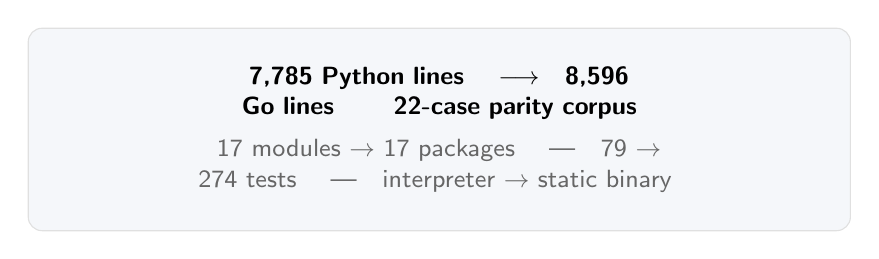
\begin{tikzpicture}
\node[
  rounded corners=5pt,
  draw=black!12,
  fill=cardbg,
  inner sep=14pt,
  text width=0.78\textwidth,
  align=center,
  font=\sffamily\small
] {
  \textbf{7,785 Python lines} \quad$\longrightarrow$\quad \textbf{8,596 Go lines} \qquad \textbf{22-case parity corpus}\\[0.45em]
  \textcolor{black!60}{
    17 modules $\rightarrow$ 17 packages \quad|\quad 79 $\rightarrow$ 274 tests \quad|\quad interpreter $\rightarrow$ static binary
  }
};
\end{tikzpicture}
\vfill
{\large\textbf{Migration Report}\par}
\vspace{0.2cm}
{\large \today\par}
\end{titlepage}

\tableofcontents
\clearpage

% ===========================================================================
\section{Background and Motivation}
% ===========================================================================

\noindent
kaal is a Go agent harness---one static binary---that runs DeepSeek~V4 Flash with tools, persistent memory, sessions, and a bubbletea TUI. It did not start as Go. Its predecessor was a Python codebase of \textbf{7,785 lines} across \textbf{17 \texttt{harness/} modules} (\textbf{13,877} lines with tests), whose only third-party dependency was Textual for the terminal UI.

Five bindings of the Python build motivated the crossing:

\begin{enumerate}[leftmargin=*,itemsep=0.35em]
  \item \textbf{TUI/loop coupling under one GIL-threaded process.} Textual's \texttt{call\_from\_thread} marshaling policed widget-thread rules that Go's event model simply does not have.
  \item \textbf{Per-thread socket juggling.} Keep-alive connections had to be scoped per thread; \texttt{--batch} workers could not share a connection. Go's \texttt{net/http.Transport} pools connections natively and a transport per worker is a dial option, not a workaround.
  \item \textbf{GIL-bound tool batches.} The $\leq 4$-worker \texttt{ThreadPoolExecutor} pools gave no true parallelism on CPU-bound scans; goroutines do.
  \item \textbf{Cooperative cancellation.} TUI Ctrl+C only \emph{asked} the worker thread to stop. Go's \texttt{context} makes it a hard, guaranteed cancel that unwinds the in-flight SSE stream.
  \item \textbf{A venv to ship.} Python needed uv + a virtualenv; Go ships one static binary with no interpreter to coax and a release-fetch self-update.
\end{enumerate}

The port was never a rewrite. The plan, recorded in \texttt{docs/go-migration-plan.md} and later narrated in the Mahabharata voice of the repository, was a deliberate, test-driven crossing: keep both camps standing until a parity gate was won, then burn the old one.

% ---------------------------------------------------------------------------
% Architecture diagram
% ---------------------------------------------------------------------------
\begin{figure}[ht]
\centering
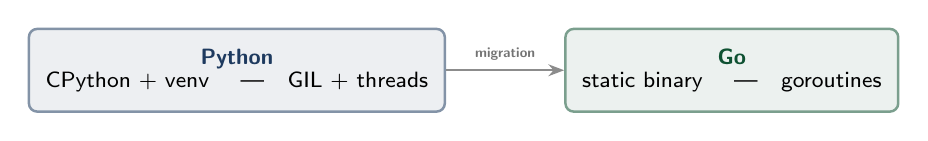
\begin{tikzpicture}[kaal, node distance=1.5cm]
  \node[archbox=pyblue] (python) {
    \textbf{\textcolor{pyblue}{Python}}\\[-1pt]
    CPython + venv \quad|\quad GIL + threads
  };
  \node[archbox=gogreen, right=1.5cm of python] (go) {
    \textbf{\textcolor{gogreen}{Go}}\\[-1pt]
    static binary \quad|\quad goroutines
  };
  \draw[arrow] (python.east) -- node[
    above, font=\sffamily\tiny\bfseries, text=black!55
  ] {migration} (go.west);
\end{tikzpicture}
\caption{The migration changed the execution model while preserving the observable harness contract.}
\label{fig:architecture}
\end{figure}

% ===========================================================================
\section{Migration Strategy: Seven Formations and a Parity Gate}
% ===========================================================================

\noindent
The campaign was fought in seven named formations over an estimated \textbf{20 person-days}. Each phase ported a slice of the army with its tests \emph{first}, so the Python tests were the ground truth for the Go implementation, never the other way around.

\begin{table}[ht]
\centering
\small
\begin{tabularx}{\textwidth}{@{}l l c Y@{}}
\toprule
\textbf{Phase} & \textbf{Name} & \textbf{Days} & \textbf{Delivered} \\
\midrule
P0 & Chakra & 1 & \texttt{go.mod}, \texttt{cmd/kaal} stub, CI matrix, release-fetch update \\
P1 & Makara & 3 & \texttt{dialect} + \texttt{messages} + \texttt{gateway}---the wire layer \\
P2 & Garuda & 4 & \texttt{AgentLoop} + tool registry, safety guards, exit codes \\
P3 & Kurma & 2 & sessions, memory, structure cache, tool cache \\
P4 & Suchi & 2 & Cobra CLI: run, batch, sessions, doctor, update, diagrams \\
P5 & Padma & 4 & Bubbletea TUI, slash commands, Markdown parity tuning \\
P6 & Krauncha & 2 & transport tuning, async persistence, parallel grep \\
P7 & Gate & 2 & parity corpus diff; Python tree deleted \\
\bottomrule
\end{tabularx}
\caption{The migration formations and their primary deliverables.}
\label{tab:formations}
\end{table}

% ---------------------------------------------------------------------------
% Minimal timeline diagram
% ---------------------------------------------------------------------------
\begin{figure}[ht]
\centering
\resizebox{\textwidth}{!}{%
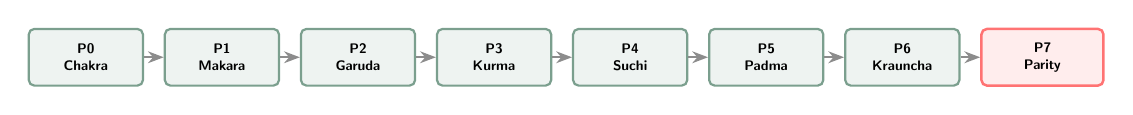
\begin{tikzpicture}[kaal, node distance=0.25cm]
  \node[phase] (p0) {P0\\Chakra};
  \node[phase, right=of p0] (p1) {P1\\Makara};
  \node[phase, right=of p1] (p2) {P2\\Garuda};
  \node[phase, right=of p2] (p3) {P3\\Kurma};
  \node[phase, right=of p3] (p4) {P4\\Suchi};
  \node[phase, right=of p4] (p5) {P5\\Padma};
  \node[phase, right=of p5] (p6) {P6\\Krauncha};
  \node[gate, right=of p6] (p7) {P7\\Parity};
  \foreach \a/\b in {p0/p1,p1/p2,p2/p3,p3/p4,p4/p5,p5/p6,p6/p7}
    \draw[arrow] (\a) -- (\b);
\end{tikzpicture}%
}
\caption{The migration sequence. P7 is the release gate, not another implementation phase.}
\label{fig:timeline}
\end{figure}

\subsection{The parity gate}
\noindent
P7 ran Python and Go binaries on the same \textbf{22-case corpus} drawn from the test fixtures and diffed the final answers, session JSONL shape, tool-call sequences, and reasoning replay on turn 2+ against each other. The gate instrument now lives in \texttt{internal/parity} and self-skips when a Python toolchain is absent. The gate was won; \texttt{harness/}, \texttt{tests/}, and the Textual dependency were deleted. kaal is Go.

% ===========================================================================
\section{Module-by-Module Mapping}
% ===========================================================================

\noindent
Every Python module became one Go package with the same duty. The numbers below are the current Go tree (\texttt{cmd/} + \texttt{internal/}), measured at the time of writing.

\begin{table}[ht]
\centering
\small
\begin{tabularx}{\textwidth}{@{}l l Y@{}}
\toprule
\textbf{Python module} & \textbf{Go package} & \textbf{Duty} \\
\midrule
\texttt{cli.py} (741) & \go{cmd/kaal} (Cobra) & command surface, exit codes 0/1/2 \\
\texttt{tui.py} (2,978) & \go{internal/tui} (Bubbletea) & terminal workbench; only Charmbracelet import \\
\texttt{loop.py} (726) & \go{internal/loop} & \texttt{AgentLoop}, \texttt{AgentEvent} seam \\
\texttt{gateway.py} (435) & \go{internal/gateway} & SSE client, $3\times$ retry, pooled transport \\
\texttt{dialect.py} (499) & \go{internal/dialect} & DSML state machine + leaked-token stripper \\
\texttt{messages.py} (105) & \go{internal/messages} & wire structs, \texttt{reasoning\_content} replay \\
\texttt{context.py} & \go{internal/context} & token estimate, history truncation \\
\texttt{tools.py} (962) & \go{internal/tools} & registry, schemas, path confinement, DENY list \\
\texttt{sessions.py} (209) & \go{internal/sessions} & JSONL store, resume replay, async writer \\
\texttt{memory.py} (152) & \go{internal/memory} & \texttt{.agent-memory} digest, caps, dedupe \\
\texttt{structure.py} (236) & \go{internal/structure} & \texttt{.kaal/STRUCTURE.md} cache \\
\texttt{toolcache.py} & \go{internal/toolcache} & read-only tool-result cache, atomic rename \\
\bottomrule
\end{tabularx}
\caption{Python-to-Go package mapping.}
\label{tab:module-map}
\end{table}

\noindent
\textbf{The dependency budget was kept.} The core (\texttt{config}, \texttt{gateway}, \texttt{dialect}, \texttt{messages}, \texttt{context}, \texttt{loop}, \texttt{prompts}, \texttt{tools}, \texttt{memory}, \texttt{sessions}, \texttt{structure}, \texttt{toolcache}) is stdlib-only and maps 1:1 to a future Rust port. Bubbletea/bubbles/lipgloss/glamour appear only in \texttt{internal/tui}; Cobra only in \texttt{internal/cli}; modernc.org/sqlite only in \texttt{internal/config} for the read-only OMP auth store. \texttt{jsonpy} reproduces Python-compatible JSON byte-for-byte for the wire, including insertion-ordered DSML arguments.

% ===========================================================================
\section{The Two Hard Things: Wire Contracts, Not Cosmetics}
% ===========================================================================

\noindent
Two properties of the system are load-bearing: drop either and the gateway misbehaves. Both were the \emph{first} arrows drawn in P1, ported with their full test tables before the implementations shipped.

\subsection{DSML Healing}
\noindent
The model does not deliver its tool calls cleanly. It emits them as a DSML XML envelope with \emph{fullwidth pipe} \textbf{U+FF5C} that leaks into the visible \texttt{delta.content} instead of arriving as structured \texttt{tool\_calls}. The \py{dialect} \texttt{DialectFeed} heals this incrementally and strips leaked chat-template tokens. The Unicode markers are load-bearing---the model was never trained on ASCII substitutes, so transliterating them breaks healing. In Go the markers are rune/string constants (\texttt{FW = "\textbackslash{}uff5c"}, \texttt{B = "\textbackslash{}u2581"}) and UTF-8-native strings simplify the logic: no surrogate-pair arithmetic, and \texttt{bytes.Contains} on the raw UTF-8 works without decoding. All 299 lines of \texttt{test\_dialect.py} became table-driven Go tests.

\subsection{\texttt{reasoning\_content} Replay}
\noindent
When an assistant turn makes tool calls, the next request \emph{must} carry that turn's streamed \texttt{reasoning\_content} verbatim; otherwise the gateway answers \textbf{HTTP 400 on turn 2+}. This is where Go's zero-value trap bites: an empty string is indistinguishable from an absent field, so the wire struct uses \texttt{ReasoningContent *string}---replay happens iff the pointer is set, never synthesized. A golden test asserts the turn-2 request body is byte-identical to the Python fixture.

% ===========================================================================
\section{Did It Affect the Inference Harness?}
% ===========================================================================

\noindent
\textbf{Semantics: no. Mechanism: yes.} The inference path---the chain from prompt to wire body to SSE stream back to resolved tool calls---was carried across with its observable contract preserved and then proven equal by the parity gate.

\begin{itemize}[leftmargin=*,itemsep=0.35em]
  \item \textbf{Wire bodies byte-identical.} \py{jsonpy} reproduces Python's separators and key order; the turn-2 request, including reasoning replay, is asserted byte-equal to the Python fixture. \texttt{encoding/json}'s sorted keys are acceptable for CLI records, never for the wire.
  \item \textbf{Forbidden fields stay forbidden.} The gateway never sends \texttt{tool\_choice}, \texttt{temperature}, \texttt{stream\_options}, or \texttt{store}. The model rejects them, so this is enforced as struct-field-absence assertions in \go{TestBuildBody}.
  \item \textbf{Retry policy preserved.} 5xx/network failures are retried up to $3\times$ with 1s/2s/4s backoff; 4xx responses fail immediately; no retry occurs after visible content. Transport is pooled (\texttt{MaxConnsPerHost}=4, idle timeout 90s); batch workers get a transport per goroutine.
  \item \textbf{Structured beats healed.} When both arrive, structured \texttt{tool\_calls} win over healed calls:
  \[
    \texttt{calls = structuredCalls if len > 0 else healedCalls}.
  \]
  The precedence was not ``fixed'' during the port.
  \item \textbf{Healing behavior identical.} \texttt{DialectFeed.Flush()} keeps its end-of-stream semantics: unclosed sections with $\geq 1$ parsed invoke are discarded; zero-invoke sections are recovered as visible text; an envelope after visible text in the same turn is prose and is never healed.
\end{itemize}

\noindent
The one deliberate inference-side \emph{improvement} is mechanism: hard \texttt{context} cancellation, so Ctrl+C truly aborts the in-flight SSE stream and unwinds the turn, replacing Python's cooperative ask.

% ---------------------------------------------------------------------------
% Contract diagram
% ---------------------------------------------------------------------------
\begin{figure}[ht]
\centering
\resizebox{\textwidth}{!}{%
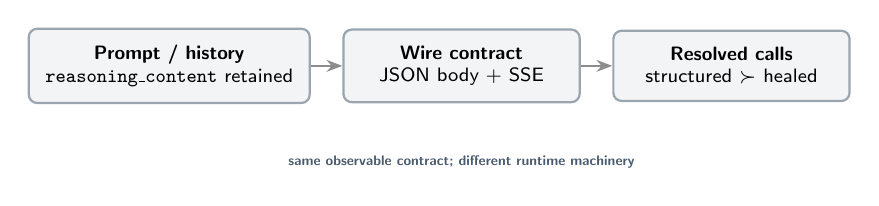
\begin{tikzpicture}[kaal, node distance=0.4cm]
  \node[seam, minimum width=3.0cm] (prompt) {
    \textbf{Prompt / history}\\
    \texttt{reasoning\_content} retained
  };
  \node[seam, right=of prompt, minimum width=3.0cm] (wire) {
    \textbf{Wire contract}\\
    JSON body + SSE
  };
  \node[seam, right=of wire, minimum width=3.0cm] (tools) {
    \textbf{Resolved calls}\\
    structured $\succ$ healed
  };
  \draw[arrow] (prompt) -- (wire);
  \draw[arrow] (wire) -- (tools);
  \node[
    below=0.55cm of wire, font=\sffamily\tiny\bfseries, text=accent
  ] {same observable contract; different runtime machinery};
\end{tikzpicture}%
}
\caption{The inference contract that the migration deliberately preserved.}
\label{fig:inference-contract}
\end{figure}

% ===========================================================================
\section{Did It Affect the Agent Harness?}
% ===========================================================================

\noindent
The agent harness---the loop, the tools, and persistence---likewise kept its contract and changed its machinery.

\begin{itemize}[leftmargin=*,itemsep=0.35em]
  \item \textbf{The \texttt{AgentEvent} stream is the port seam.} The TUI and \texttt{kaal run} both consume exactly this typed event stream (\texttt{content}, \texttt{reasoning}, \texttt{tool\_start}, \texttt{tool\_result}, \texttt{verify}, \texttt{step}, \texttt{done}, \texttt{error}). It was preserved byte-for-byte so the front end was a consumer swap, not a rewrite. \go{internal/loop} owns the whole turn on its own goroutine; the TUI subscribes via Bubbletea's standard channel pattern, so there are no widget-thread rules to police.
  \item \textbf{Parallel tool batches.} All-read batches (\texttt{read}/\texttt{grep}/\texttt{glob}) run concurrently under a semaphore capped at four workers; any batch containing a mutator, \texttt{ask\_user}, or a spawn runs serially in call order. Events, persistence, tool-loop detection, and failure counting are recorded in call order on the main goroutine.
  \item \textbf{Tool safety carried over verbatim.} Path confinement (\texttt{filepath.Rel} + prefix check), the destructive command DENY list, the 10k-rune result cap, bash timeout (30s default / 300s maximum via \texttt{exec.CommandContext}), 1-based \texttt{read} offset, and the rg-backed grep with a pure-Go parallel fallback were all ported with the 556 lines of \texttt{test\_tools.py} cases.
  \item \textbf{Loop governance unchanged.} Tool-loop detection, the five-consecutive-failure abort, and exit-code mapping (0 answer / 1 config-key-gateway / 2 loop) were reproduced. The ``empty answer is an answer'' distinction (turn-done vs.\ continue) was kept.
  \item \textbf{Persistence hardened, not just ported.} Sessions went from per-thread appends to a single \texttt{AsyncWriter} per process with flush-on-turn-end, so the JSONL store is durable when \texttt{Run} returns. The tool-result cache is signature-keyed: a changed tree automatically misses.
  \item \textbf{Nested agents.} \texttt{spawn\_agent} / \texttt{spawn\_parallel\_task} became goroutines with an atomic depth counter (cap 2), \texttt{allow\_dangerous=false}, and no tool cache---exactly as today.
\end{itemize}

% ===========================================================================
\section{Results and Quantification}
% ===========================================================================

\begin{table}[ht]
\centering
\small
\begin{tabularx}{\textwidth}{@{}Yrr@{}}
\toprule
\textbf{Metric} & \textbf{Python} & \textbf{Go} \\
\midrule
Source lines (non-test) & 7,785 (17 modules) & 8,596 (17 packages, 35 files) \\
Lines with tests & 13,877 & 16,450 \\
Runtime dependency budget & Textual (only dependency) & Bubbletea family (TUI only) \\
Interpreter / runtime & CPython + venv & static binary, zero runtime \\
Concurrency primitive & \texttt{ThreadPoolExecutor}, GIL & goroutines, channels, \texttt{context} \\
Cancellation & cooperative & hard (\texttt{context.WithCancel}) \\
Tests (count) & 79 unit & 274 (all green under \texttt{go test -race}) \\
Parity evidence & --- & 22-case corpus, both armies diffed \\
\bottomrule
\end{tabularx}
\caption{Old versus new, in numbers.}
\label{tab:results}
\end{table}

\noindent
The port shipped with a clean bill of health: \texttt{go build} clean, \texttt{go test -race ./...} green across all 17 packages, and \texttt{go vet} clean. A \texttt{kaal doctor} self-check exercises the Go toolchain, terminal, API key, gateway, structure cache, and sessions directory.

% ---------------------------------------------------------------------------
% Result summary diagram
% ---------------------------------------------------------------------------
\begin{figure}[ht]
\centering
\begin{tikzpicture}[kaal, node distance=0.8cm]
  \node[archbox=pyblue, minimum width=3.4cm] (old) {
    \textbf{Python}\\
    7,785 source lines\\
    79 unit tests
  };
  \node[
    circle,
    draw=black!25,
    fill=cardbg,
    line width=0.7pt,
    minimum size=0.75cm,
    font=\sffamily\small\bfseries
  ] (arrow) at ($(old.east)!0.5!(new.west)$) {$\rightarrow$};
  \node[archbox=gogreen, minimum width=3.4cm, right=2.6cm of old] (new) {
    \textbf{Go}\\
    8,596 source lines\\
    274 tests + race detector
  };
  \node[
    below=0.6cm of arrow, font=\sffamily\tiny, text=black!55
  ] {22-case parity gate};
\end{tikzpicture}
\caption{The migration increased implementation and test surface while removing the interpreter/runtime dependency.}
\label{fig:results}
\end{figure}

% ===========================================================================
\section{Lessons Learned}
% ===========================================================================

\begin{enumerate}[leftmargin=*,itemsep=0.4em]
  \item \textbf{Test tables first, implementation second.} Porting the Python test tables before writing Go code made the old tests the ground truth and caught drift at unit level. The turn-2 reasoning-replay golden test is the canonical example.
  \item \textbf{Load-bearing markers must survive as constants, not glyphs.} The Unicode markers (U+FF5C, U+2581) are matched exactly and fixtures are built from escapes---never paste the glyphs.
  \item \textbf{A port seam pays for itself.} The \texttt{AgentEvent} channel decoupled the loop from the UI, making the 2,978-line TUI a consumer swap rather than a rewrite.
  \item \textbf{Go's zero-value is a wire hazard.} \texttt{ReasoningContent} had to be a pointer; an empty string is not an absent field.
  \item \textbf{The parity gate earns its keep once.} The instrument self-skips without a Python toolchain, but the discipline of running both armies on the same corpus is what made the burn safe.
\end{enumerate}

% ===========================================================================
\section{Conclusion}
% ===========================================================================

\noindent
The crossing to Go is complete and verified. The inference and agent harnesses were affected in mechanism and deliberately \emph{not} affected in observable contract: the wire bytes, the healing rules, the reasoning replay, the retry policy, the event stream, and the safety boundaries all survived the crossing and were diffed equal on a 22-case corpus before the Python camp was burned. kaal is now one static binary---no venv, no interpreter, hard cancellation, and a future that maps package-for-package onto an eventual Rust port.

\end{document}
